\documentclass[main.tex]{subfiles}
\begin{document}
\begin{figure}[htbp]
	\centering
	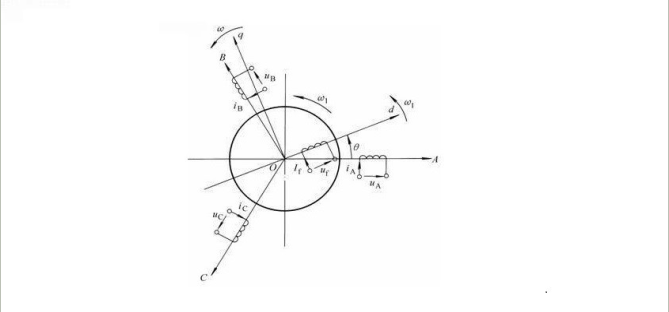
\includegraphics[width=0.75\textwidth]{img/img_1.1.png}
\end{figure}
\section{经典FOC算法}
FOC框图及仿真参见\href{https://github.com/Ding-Kaiyue/FOC_Simulation}{FOC simulation based on Matlab 2020a}
\subsection{电压平衡方程}
电机磁场的分布由电机结构决定。当定子绕组的导体沿圆周正弦分布时,通入任意电流都能得到正弦分布的磁场,通入电流仅决定正弦磁场幅值和角度的变化规律。

转子磁场的分布由永磁体和磁路决定;气隙磁场由定子磁场和转子磁场合成而来。如果二者均为正弦分布且磁路线性,那么合成磁场依然位正弦分布。

气隙磁场是否正弦,对电压平衡方程的得出没有影响,对于理想电机,以下公式总是成立。扩展到BLDC电机,其电压平衡方程也是这个形式。
\[
	u_{3s} = R_{3s}\dot i_{3s} + d\psi_{3s}/dt	
\]

物理量是否正弦不影响Clark变换和Park变换的应用,只不过非正弦变换后Iq, Id不是直流量。

\subsection{三相PMSM坐标变换}
\begin{figure}[H]
	\centering
	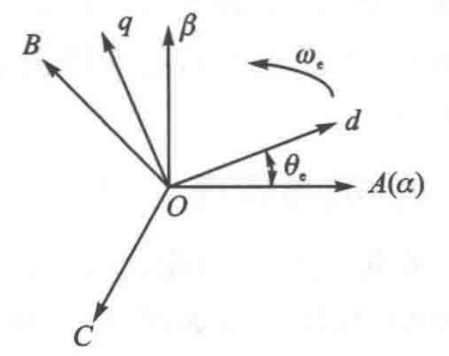
\includegraphics[width=0.35\textwidth]{img/img_1.1.1.png}
	\caption{各坐标系之间的关系}
	\label{各坐标系之间的关系}
\end{figure}
图\ref{各坐标系之间的关系}表示了\emph{ABC三相自然坐标系,$\alpha-\beta$两相静止坐标系和d-q两相旋转坐标系}\footnote{参见稚晖君FOC入门文章}及电机旋转电角度及电角速度。

\subsubsection{自然坐标系和$\alpha-\beta$静止坐标系转换 —— Clark变换}

将$I_a,I_b, I_c$正交化为一个直角坐标系,如式\ref{Clark Transform}所示,该式为Clark变换的表达式:

\begin{equation}
\begin{bmatrix}
	I_\alpha\\
	I_\beta
\end{bmatrix}
=
\begin{bmatrix}
	1 & -\frac{1}{2} & -\frac{1}{2}\\
	0 & \frac{\sqrt{3}}{2} & -\frac{\sqrt{3}}{2}
\end{bmatrix}
\begin{bmatrix}
	I_a\\
	I_b\\
	I_c
\end{bmatrix}
\label{Clark Transform}
\end{equation}

\subsubsection{静止坐标系和旋转坐标系转换 —— Park变换}

将$\alpha-\beta$坐标系旋转$\theta$度,$\theta$是转子当前的角度,变换公式如式\ref{Park Transform}所示,该式为Park变换的表达式:

\begin{equation}
\begin{bmatrix}
	I_d\\
	I_q
\end{bmatrix}
=
\begin{bmatrix}
	\cos\theta & \sin\theta \\
	-\sin\theta & \cos\theta
\end{bmatrix}
\begin{bmatrix}
	I_\alpha\\
	I_\beta
\end{bmatrix}
\label{Park Transform}
\end{equation}

\subsubsection{旋转坐标系和静止坐标系转换 —— 逆Park变换}
将式\ref{Park Transform}求逆即可得到逆Park变换的公式\ref{Rev Park Transform}

\begin{equation}
\begin{bmatrix}
	I_\alpha\\
	I_\beta
\end{bmatrix}
=
\begin{bmatrix}
	\cos\theta & \sin\theta \\
	\sin\theta & \cos\theta
\end{bmatrix}
\begin{bmatrix}
	I_d\\
	I_q
\end{bmatrix}
\label{Rev Park Transform}
\end{equation}

\subsection{电机初始定位}
一般将转子磁极方向和$\alpha$轴(A轴)正向重合的位置作为转子零位(转子在此位置时角度为0°),然后根据控制算法依据FOC产生一个超前90°的电流is来拖动电机转起来。

上电时编码器初始为0,但是转子位置是随机的,假设为125°,但控制算法不知道此时位置为125°,依然人为此时是0°,然后根据FOC产生一个90°的q轴电流,这时会吸引转子反向转起来。转子转了多少度,编码器也增加了多少度,但两者之间始终差了一个125°,所以转子会一直转下去。故在正常运行之前要将编码器和转子位置角度重合起来,也就是电机初始定位。

实现方法:控制算法在刚上电时产生一个固定为0°的电流,转子在这个电流产生的定子磁场的吸引下就会转起来,这个定子磁场方向是固定的,转子就被吸引到0°的位置固定下来,然后在这个位置将编码器计数值初始为0即可后续根据实际编码器角度做控制。

\begin{lstlisting}[language=C]
    foc->Volt.Vq = 0.0f;
    foc->Volt.Vd = 0.05f;
    foc->cos_theta = 1.0f;
    foc->sin_theta = 0.0f;
    InvPark_Transform(foc);
    SVPWM_Calc(foc);
\end{lstlisting}

\subsection{空间电压矢量及SVPWM算法简介}

SVPWM算法的目的,就是使用逆变器三相桥的开关状态把在空间中旋转的矢量表示出来,这个矢量称为空间电压矢量。

假设三相对称正弦相电压的瞬时值为
\begin{equation}
\begin{aligned}
	u_a &= U_m\cos\omega t \\
	u_b &= U_m\cos(\omega t - \frac{2}{3}\pi) \\
	u_c &= U_m\cos(\omega t + \frac{2}{3}\pi)
\end{aligned}
\end{equation}

电压矢量$\textbf{U}_{out}$的实部和虚部为
\begin{equation}
\begin{aligned}
	Re\textbf{U}_{out} &=  u_a+u_b\cos\frac{2}{3}\pi+u_c\cos{(-\frac{2}{3}\pi)} = \frac{3}{2}U_m\sin\omega t	 \\
	Im\textbf{U}_{out} &= u_b\sin\frac{2}{3}\pi+u_c\sin(-\frac{2}{3}\pi) = -\frac{3}{2}U_m\cos\omega t
\end{aligned}
\end{equation}

空间电压矢量为
\begin{equation}
	\textbf{U}_{out} = Re\textbf{U}_{out} + jIm\textbf{U}_{out} = \frac{3}{2}U_me^{j(\omega t-\frac{\pi}{2})}
\end{equation}

可以知道空间电压矢量的运动轨迹为一个圆,且以角速度$\omega$逆时针旋转,则原三相电压越趋近于三相对称正弦波。\emph{逆变器}\footnote{逆变器由三路逆变桥组成,每路逆变桥有上下两个桥臂,上下开关器件不能同时导通,故逆变器的开关组态共$2^3$种,这8种组态可以得到8个基本空间电压矢量,通过pwm技术可以将两个线性无关的矢量合成为轨迹上任意一点}交流输出电压的控制目标就是输出完美的三相对称正弦波,通过空间矢量变换,可以将逆变器三相输出的三个标量的控制问题转换为一个矢量的控制问题。

8个基本空间电压矢量映射到复平面如图\ref{空间电压矢量图}所示,它们将复平面划分成了6个扇区。通过判断空间电压矢量所在的扇区,可以选择不同的两个基向量使用PWM技术来合成该扇区内任意空间电压矢量。

\begin{figure}[H]
	\centering
	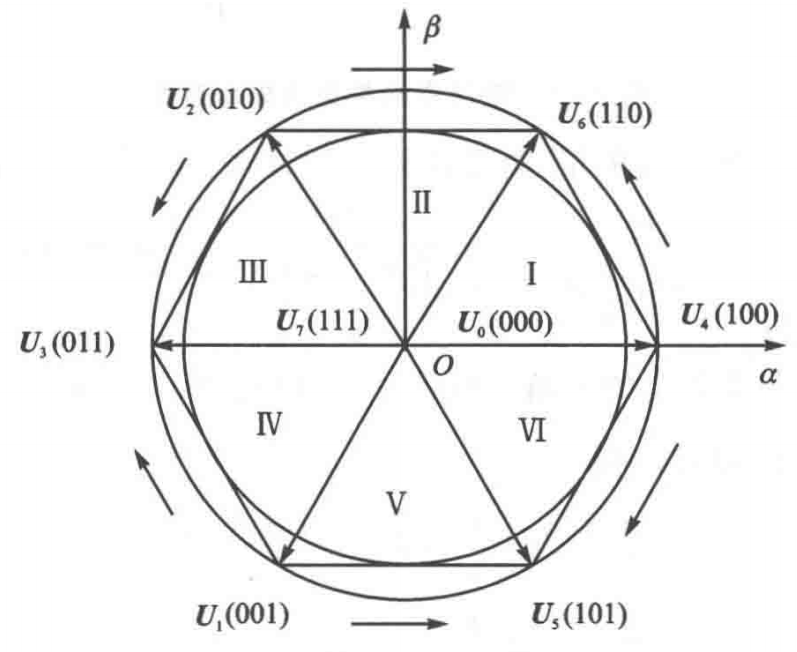
\includegraphics[width=0.35\textwidth]{img/img_1.1.2.png}
	\caption{空间电压矢量图}
	\label{空间电压矢量图}
\end{figure}

\subsection{SVPWM算法的实现}

\subsubsection{参考电压矢量扇区判断}

用$U_\alpha$和$U_\beta$表示参考电压矢量在$\alpha-\beta$轴上的分量,定义
\begin{equation}
\begin{aligned}
	U_{ref1} &= u_\beta \\
	U_{ref2} &= \frac{\sqrt{3}}{2}u_\alpha - \frac{1}{2}u_\beta \\
	U_{ref3} &= -\frac{3}{2}u_\alpha - \frac{1}{2}u_\beta
\end{aligned}
\end{equation}

定义A=1(if $U_{ref1} > 0$), B=1(if $U_{ref2} > 0$), C=1(if $U_{ref1} > 0$), 否则为0。令$N=4C+2B+A$可以得到与扇区的关系如表\ref{N与扇区的关系}所示:
\begin{table}[H]
	\centering
	\begin{tabular}{|c|c|c|c|c|c|c|}
	\bottomrule
	N & 3 & 1 & 5 & 4 & 6 & 2	\\
	\hline
	扇区 & \uppercase\expandafter{\romannumeral1} & \uppercase\expandafter{\romannumeral2} & 
	\uppercase\expandafter{\romannumeral3} & \uppercase\expandafter{\romannumeral4} & 
	\uppercase\expandafter{\romannumeral5} & \uppercase\expandafter{\romannumeral6} \\
	\toprule
	\end{tabular}
	\caption{N与扇区的关系}
	\label{N与扇区的关系}
\end{table}

\subsubsection{非零矢量和零矢量作用时间的计算}

由图\ref{空间电压矢量图}可知,以扇区I内的空间电压矢量为例,$\textbf{U}_{out}$可以分解成式\ref{扇区I分解}:

\begin{equation}
\begin{aligned}
	u_\alpha &= \frac{T_4}{T_s}|\textbf{U}_4|+\frac{T_6}{T_s}|\textbf{U}_6|\cos\frac{\pi}{3}\\
	u_\beta &= \frac{T_6}{T_s}|\textbf{U}_6|\sin\frac{\pi}{3}\\
\end{aligned}
\label{扇区I分解}
\end{equation}

那么由$\u_\alpha$和$\u_\beta$的值可以判断$\textbf{U}_{out}$位于哪个扇区对应的N。同样以扇区I为例,由式\ref{扇区I分解}可以推出$U_4$和$U_6$的作用时间$T_4$和$T_6$如式\ref{扇区I内两个基向量作用时间}所示:

\begin{equation}
\begin{aligned}
	T_4 &= \frac{\sqrt{3}T_s}{2U_dc}(\sqrt{3}u_\alpha-u_\beta)	\\
	T_6 &= \frac{\sqrt{3}T_s}{2U_dc}u_\beta \\
\end{aligned}
\label{扇区I内两个基向量作用时间}
\end{equation}

令

\begin{equation}
\begin{aligned}
	X &= \frac{\sqrt{3}T_s u_\beta}{U_{dc}}	\\
	Y &= \frac{\sqrt{3}T_s}{U_{dc}}(\frac{\sqrt{3}}{2}u_\alpha + \frac{1}{2}u_\beta)	\\
	Z &= \frac{\sqrt{3}T_s}{U_{dc}}(-\frac{\sqrt{3}}{2}u_\alpha + \frac{1}{2}u_\beta) \\
\end{aligned}
\end{equation}

各个扇区$T_0(T_7), T_4$和$T_6$作用的时间如表\ref{各扇区作用时间}所示:
\begin{table}[H]
	\centering
	\begin{tabular}{|c|c|c|c|c|c|c|}
	\bottomrule
	N & 1 & 2 & 3 & 4 & 5 & 6	\\
	\hline
	$T_4$ & Z & Y & -Z & -X & X & -Y \\
	\hline
	$T_6$ & Y & -X & X & Z & -Y & -Z \\
	\hline
	$T_0(T_7)$ & \multicolumn{6}{c|}{$T_0(T_7) = (T_s-T_4-T_6)/2$}\\
	\toprule
	\end{tabular}
	\caption{各扇区作用时间}
	\label{各扇区作用时间}
\end{table}

\subsubsection{过调制处理}

为避免$T_4$和$T_6$超过了PWM计数周期,需要进行过调制处理:

\begin{equation}
\begin{aligned}
	T_4 = \frac{T_4}{T_4+T_6}T_s \\
	T_6 = \frac{T_6}{T_4+T_6}T_s \\
\end{aligned}
\end{equation}

\subsubsection{七段SVPWM扇区矢量切换点}

定义

\begin{equation}
\begin{aligned}
	T_a &= (T_s-T_4-T_6)/4 \\
	T_b &= T_a+T_4/2		\\
	T_c &= T_b+T_6/2		\\
\end{aligned}
\end{equation}

三相电压开关时间切换点$T_{cm1}, T_{cm2}, T_{cm3}$与各扇区的关系如表\ref{各扇区时间切换点}所示:

\begin{table}[H]
    \centering
    \begin{tabular}{c|c|c|c|c|c|c}
         \bottomrule
         N & 1 & 2 & 3 & 4 & 5 & 6 \\
         \hline
         $T_{cm1}$ & $T_b$ & $T_a$ & $T_a$ & $T_c$ & $T_c$ & $T_b$ \\
         \hline
         $T_{cm2}$ & $T_a$ & $T_c$ & $T_b$ & $T_b$ & $T_a$ & $T_c$ \\
         \hline
         $T_{cm3}$ & $T_c$ & $T_b$ & $T_c$ & $T_a$ & $T_b$ & $T_a$ \\
         \toprule
    \end{tabular}
    \caption{各扇区时间切换点$T_{cm1}, T_{cm2}, T_{cm3}$}
    \label{各扇区时间切换点}
\end{table}

将以上三个值赋给定时器的影子寄存器,即可完成电机FOC控制。









\end{document}